% !TeX spellcheck = ru_RU
% !TEX root = vkr.tex

\newcolumntype{C}{ >{\centering\arraybackslash} m{4cm} }
\newcommand\myvert[1]{\rotatebox[origin=c]{90}{#1}}
\newcommand\myvertcell[1]{\multirowcell{5}{\myvert{#1}}}
\newcommand\myvertcelll[1]{\multirowcell{4}{\myvert{#1}}}
\newcommand\myvertcellN[2]{\multirowcell{#1}{\myvert{#2}}}

\afterpage{
    \clearpage
    \thispagestyle{empty}
    \begin{landscape}
        \centering
        \begin{figure}
            \begin{tabular}{cc}
                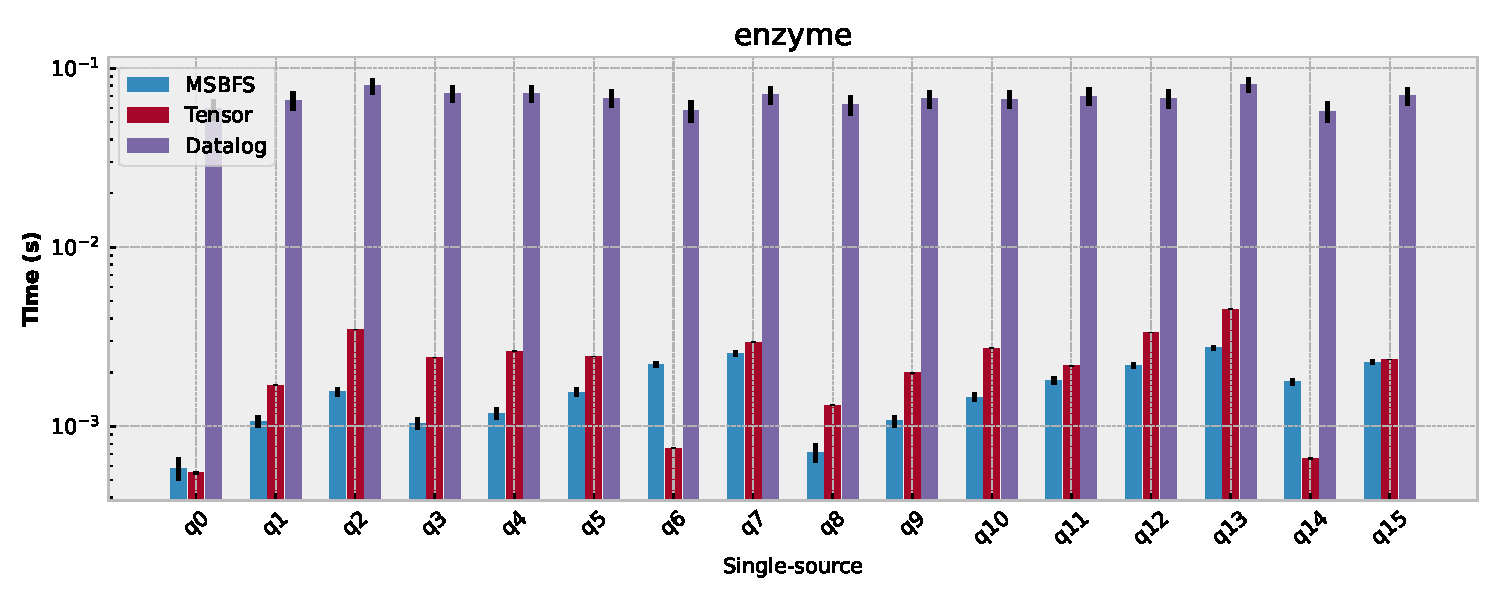
\includegraphics[width=120mm]{pictures/enzyme_ss.pdf} & 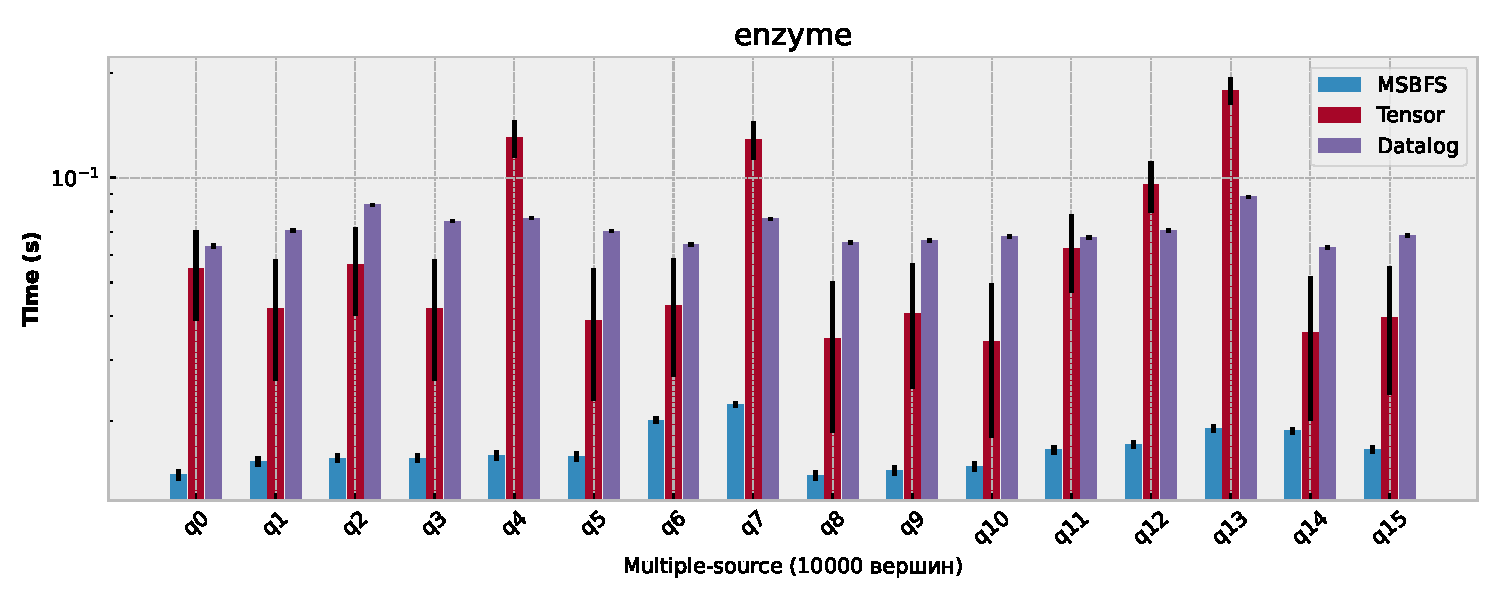
\includegraphics[width=120mm]{pictures/enzyme_ms10000.pdf} \\
                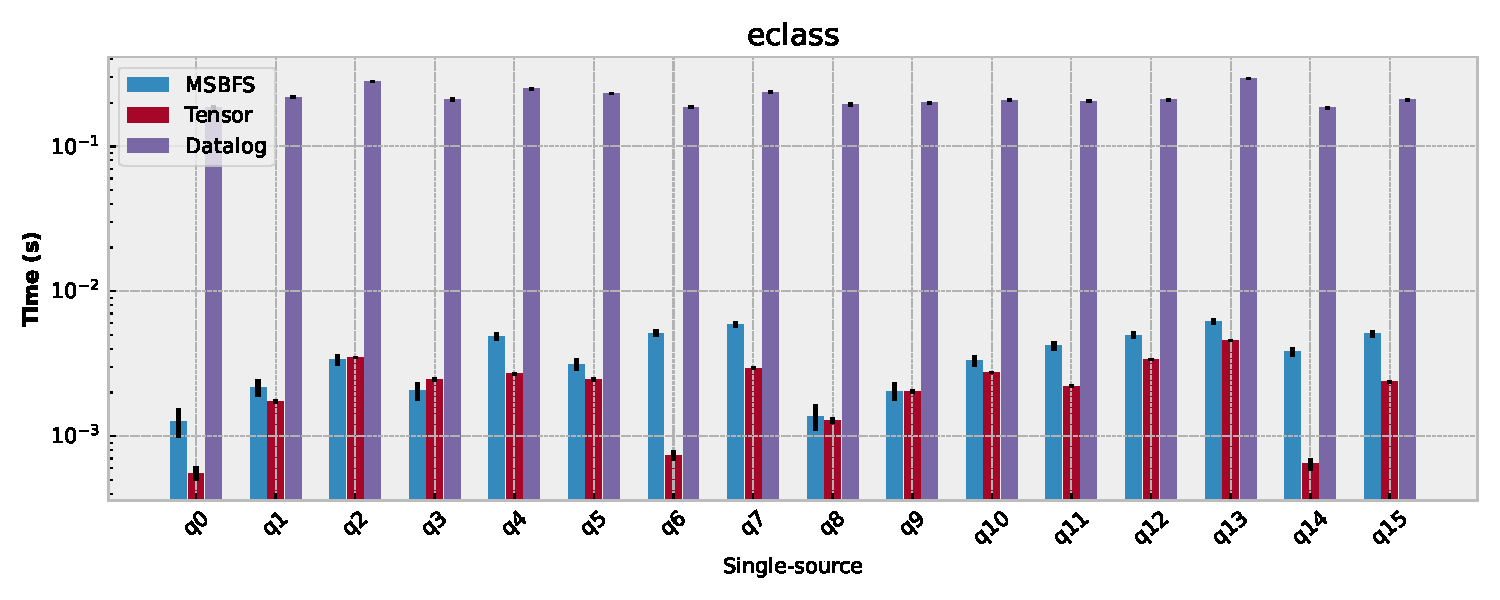
\includegraphics[width=120mm]{pictures/eclass_ss.pdf} & 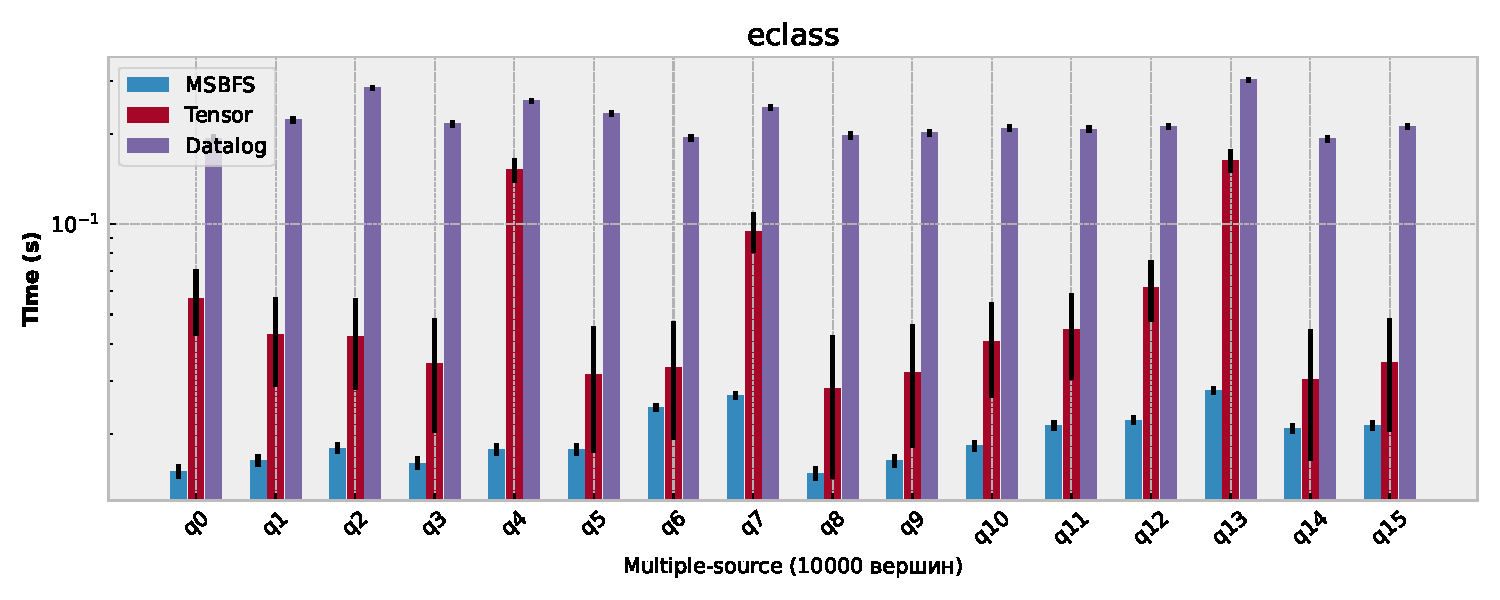
\includegraphics[width=120mm]{pictures/eclass_ms10000.pdf} \\
                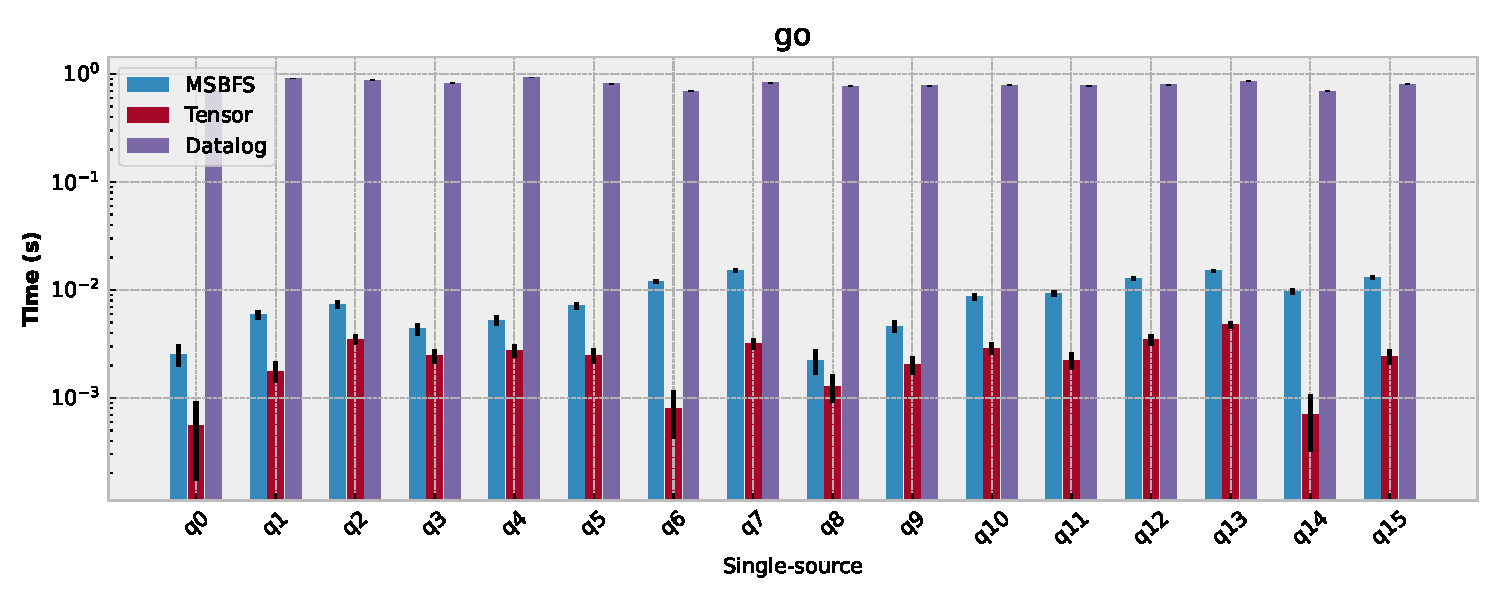
\includegraphics[width=120mm]{pictures/go_ss.pdf}     & 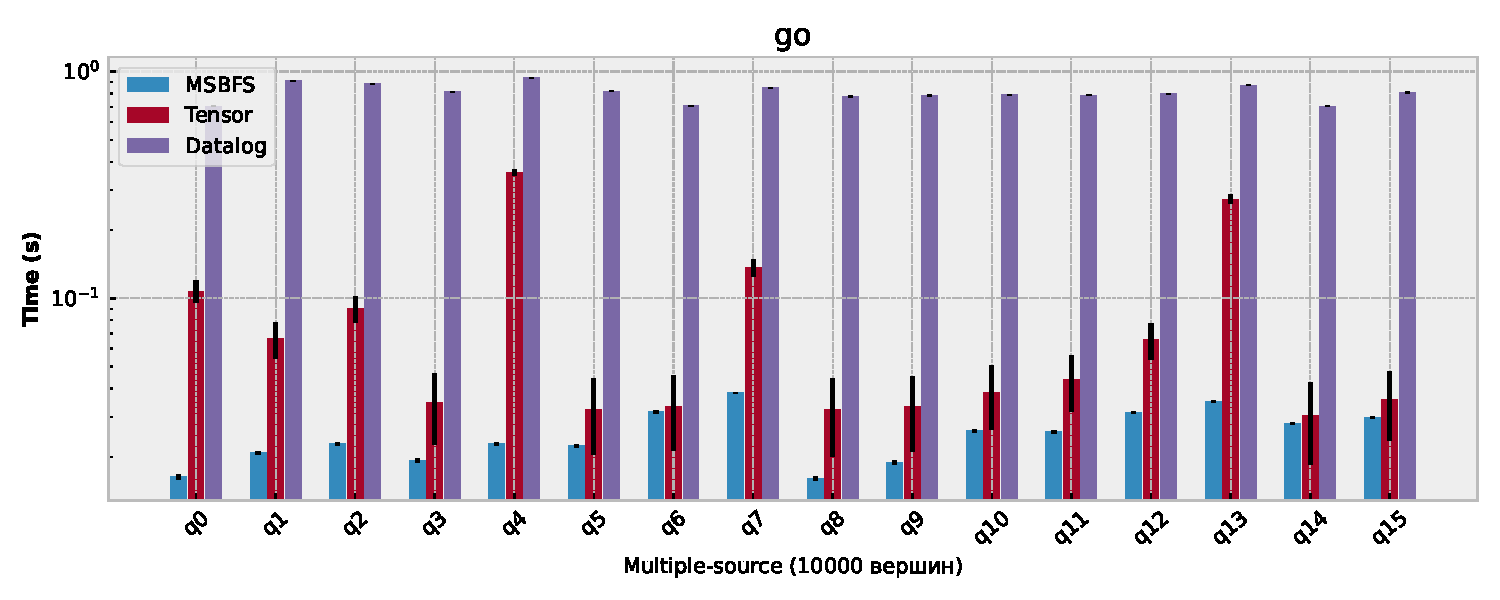
\includegraphics[width=120mm]{pictures/go_ms10000.pdf}     \\
            \end{tabular}
            \caption{Результаты эксперимента на наборе RDF-данных для single-source и multiple-source (10000 вершин) запросов.}
        \end{figure}
    \end{landscape}
    \clearpage
}
